\section{Video System}
At first glance the video output system, the VGA (Video Graphic Array), was still the same weird beast Wolfenstein 3D had to deal with. With its infamous 50 registers to configure, its palette system limiting colors to 256, and the awkward four banks of 64 KiB mandating interleaved framebuffer, the VGA was an unappealing programming interface.\\
\par
A GC (Graphic Controller) and a (SC) Sequence Controller controlled access to 256 KiB of Video RAM. A CRTC (Cathode Ray Tube Controller) controlled how the framebuffer was sampled. Finally, a DAC converted digital levels to analog levels for output to a CRT.\\
\par 	
\scaleddrawing{0.6}{vga}{}
\par
During the early 90s, a vast majority of PC video games used the VGA in tweaked mode 13h (also called Mode-Y) which offered a resolution of 320x200, 1 byte per pixel, 256 colors palette. Using this undocumented mode, developers manipulated the four banks in the video card directly. How the framebuffer was laid out across banks was far from trivia. As figure \ref{vga_ram_screen_layout} shows, due to historically slow RAM access times, pixels were interleaved four by four.




\cscaledimage{0.95}{vga_ram_screen_layout}{\label{vga_ram_screen_layout}}
\par

Notice how the first pixel \cw{0} is stored in bank 0, pixel \cw{1} is stored in bank 1 and so on. With an horizontal resolution of 320 lines, 80 non horizontally adjacent yet vertically adjacent pixels are stored in each banks.\\
\par
To access the 256 KiB of VRAM, IBM had established a hard-coded memory mapping in RAM from \cw{0xA0000} to \cw{0xAFFFF}. An eye accustomed to hexadecimal will have immediately noticed that \cw{0xFFFF} translates to 64KiB addresses, far fewer than the total available VRAM.\\
\par
 To compensate for the lack of addresses, IBM designed a bank switching system managed through a \textit{map mask register}. In practice this meant a RAM address within \cw{0xA0000} to \cw{0xAFFFF} could correspond to four locations in VRAM as shown in figure \ref{ram_vram_mapping}. The mask was cumbersome but allowed magic such as writing four pixels in one write operations\footnote{VGA mask tricks are discussed in \it{Game Engine Black Book: Wolfenstein 3D}.}.



\scaleddrawing{0.7}{vga_mapping}{\label{ram_vram_mapping}} \label{vga_ratio}
\par
\vspace{-2mm}
Another diffculty to deal with came from the different aspect ratio of mode Y framebuffer layout and the CRT display which resulted in distortions. \\
\par
\cfullimage{circleframebuffer.png}{\label{circle_framebuffer}}
\par
In figure \ref{circle_framebuffer} a programmer drew a circle into the framebuffer, notice the $ 320/200 = 1.6 $ aspect ratio.\\
\par
\cfullimage{circlescreen.png}{}
\par
Figure \ref{circle_framebuffer} shows what the same framebuffer looked like when displayed on the monitor. Notice the $ 320/240 = 1.333 $ aspect ratio.\\







\section{Hidden improvements}
Despite this bleak description, a closer inspection of the world of graphic cards unveiled two tremendous changes which ended up deeply impacting \doom. \\
\par
Since 1992 with the released of Microsoft and IBM new operating systems (respectively Microsoft Windows 3.1 and OS/2 2.0), demand for fast graphic cards had been growing strong. It was a huge technological leap to request devices pushing 4,000 bytes of information\footnote{2,000 bytes for the characters, and 2,000 bytes for screen attributes} in text mode to instead move 147,200 bytes\footnote{16 colors at 640x480} for GUIs.

\fullimage{Windows311workspace.png}\\
\par 
Despite its simple interface, Windows 3.11 640x480, 16 colors was able to put PCs on their knees. Moving a window was done via its outlines since no hardware was capable of refreshing the screen fast enough in order to also show the content\footnote{\NeXT workstations could do it and Steve Jobs mentioned it often during demos :)!}.



\subsection{VGA Chip manufacturer}
The first improvement came from VGA chip manufacturers. Sensing that demand for performance was growing, companies such as ATI, Cirrus Logic, and Tseng Labs went through great effort to compete and achieve higher performance. Hardware GUI acceleration had not yet become mainstream so host-throughput was the dominating factor in a graphical-application's redraw speed. They started to tightly integrate every component of a VGA card into a single chip (RAM, RamDAC, BIOS, Memory controller, Blitter, Ram Refresh, Cache controller, Timing Sequencer\footnote{Tseng Labs ET4000} to name only a few).\\
\par
Some manufacture such as Cirrus Logic even adopted a fabless business model where they sold semiconductor designs while outsourcing the fabrication.


An optimization among many other was to leverage the fact that VGA RAM was often subject to write operations instead of read. Using a FIFO SDRAM cache to buffer operations and return right away tremendously improved screen bliting. Peeking at a card based on one of the most notorious manufacturer of the era (Tseng Labs's), the ET4000 give a good overview of what a customer could purchase.\\ 
\par
\cfullimage{vlb_cards/tseng_lans_et4000_w32_vesa_local_illetw32.png}{ILLETW32 Britek Electronics. Photo courtesy \cw{http://www.amoretro.de/}}
\par
By licensing the ET4000 (\circled{1}), Britek Electronics only had to provide RAM(\circled{2}), RAMDAC(\circled{3}), a Timer(\circled{4}) and apply a few customization via a Programmable Array Logic TIBPAL16L8 (\circled{5}). The VGA BIOS chip (\circled{6}) could also be purchased from Tseng Labs.\\
\par
\vspace{10pt}
\drawing{vga_vlb_arch}{}

\par



\subsection{VL-Bus}
As much as the video card manufacturer could optimize their product, there was still a huge bottleneck that was out of their control. Information written by the CPU still had to transit via the ISA bus.\\
\par
 Introduced in 1981, the first incarnation of the ISA bus had an 8-bit data path running at 4.77 MHz. It was upgraded in 1984, bringing its width to 16 bits and running at 6 MHz. After 10 years of service it was starting to show its age and was considered a performance killer.\\
\par
\drawing{bus_isa}{ISA Bus}
\par
Fed up with the state of things, hardware manufacturer teamed together to form the VESA (Video Electronics Standards Association) and created a new Bus standard. They did not go for something complicated, the protocol was exactly the Intel 486 Bus Unit protocol which made it a frictionless medium.\\
\par 
The VLB doubled the bus data line of the ISA to 32 bits and increased its frequency to 33 Mhz, making the VL-Bus up to 10x faster when compared to the lowest ISA bus.\\
\par
The chip design for the VLB controller was relativity simple because many of the core instructions (Interrupts and port-mapped I/O) were still hosted by the ISA circuits already on the motherboard while memory-mapped I/O and DMA data path were on the same local bus as the one used by the CPU (see figure \ref{bus_vlb}). The speed of the system data bus was based on the clock rate of the motherboard's crystal which meant the bus ran at the same speed as the CPU.\\
\par
\drawing{bus_vlb}{VLB Bus}
\label{vlbarchitecture}

\par
The close tie of the VL-Bus architecture to the 486 Bus Unit brought unmatched performances and considerably facilitated adoption since there was no need for a chipset. The term 'local bus' meant that the address, data and control signals were directly connected to the processor so devices on the bus were connected via nothing more than some electrical buffering. This is one of the reasons for its simplicity, but it is also the reason for many of its limitations.\\
\par
Forced to run at the same speed as the CPU, the VL-Bus suffered instability as frequencies reached 40 Mhz, resulting in crashes. Past this speed, the system became increasingly intolerant to timing variations\footnote{The issue did not affect 486 DX-66Mhz which bus ran at only 33Mhz.}. The root problem is that a local bus is by definition synchronous. Expansion card vendors had the difficult task of ensuring their products could run at a range of speeds. The upper limit of the range being undefined as new processors were introduced. This was a recipe for compatibility problems\footnote{Such problems have been experienced by users of VL-Bus systems using the AMD 80MHz processors, which had a 40MHz bus clock.}.\\
\par
The second problem was that the electrical load driven by the CPU on the bus decreased as the clock speed increases. Three slots could be provided at 33MHz, but only two at 40MHz and just one at 50MHz. This resulted in configuration hell since motherboards speed was configurable and came with three slots. Users would find out some VLB slots "did not work" or "stopped working" as they tuned the frequency.\\
\par
Cards were also hard to install due to their length and required pressure to force them into the VLB slot resulting in physical breakages\footnote{Friends jokingly renamed VLB to "Very Long Bus".}.\\
\par
  Worse than everything, Intel's 1993 Pentium Bus Unit protocol changed to use the PCI which was entirely incompatible. Unable to adapt, the VL-Bus found itself obsolete and the standard died shortly after.\\
\par

\begin{figure}[H]
\centering
  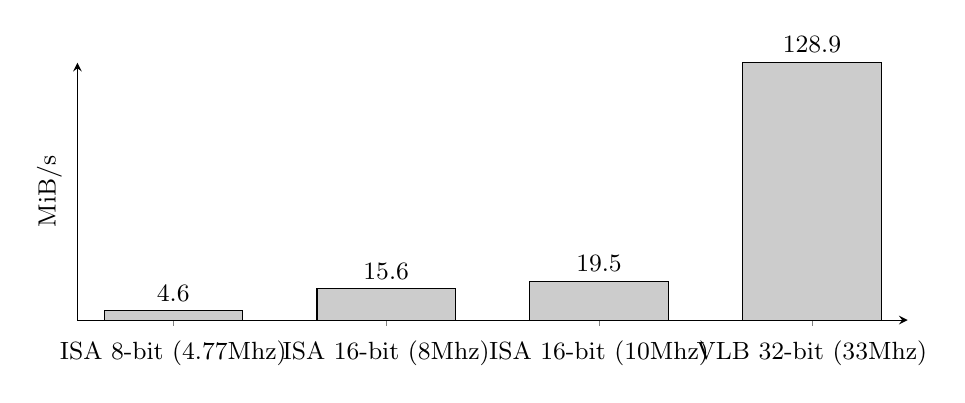
\begin{tikzpicture}[font=\small]
    \begin{axis}[
      width=1.0\textwidth,
      height=0.4\textwidth,
      ybar,
      bar width=50pt,
      ylabel={MiB/s},
      ymin=0,
      ytick=\empty,
      xtick=data,
      axis x line=bottom,
      axis y line=left,
      enlarge x limits=0.15,
      symbolic x coords={ISA 8-bit (4.77Mhz), ISA 16-bit (8Mhz),ISA 16-bit (10Mhz), VLB 32-bit (33Mhz)},
      xticklabel style={anchor=base,yshift=-\baselineskip},
      nodes near coords={\pgfmathprintnumber\pgfplotspointmeta}
    ]
      \addplot[fill=black!20,draw=black] coordinates {
        (ISA 8-bit (4.77Mhz),4.6)
        (ISA 16-bit (8Mhz),15.6)
        (ISA 16-bit (10Mhz),19.5)
        (VLB 32-bit (33Mhz), 128.9)
      };
    \end{axis}
   
   \end{tikzpicture}
   \caption{Theoretical Maximum Speeds (MiB/sec)\protect\footnotemark.}
 \end{figure}
\par
\footnotetext{At least one cycle is used to place the address on the bus which halves payload bandwidth.}
% VL-Bus design specifications provides two other performance-boosting features: burst mode and bus mastering. In burst mode, VLB devices gain complete control of the external data bus for up to four bus cycles, passing up to 16 bytes of data in a single burst (which was conveniently exactly the size of a 486 cacheline). Bus mastering allows the VLB controller to arbitrate data transfers between the external data bus and up to three VLB devices without assistance from the CPU.\\
% \par
On the opposite page, three VGA cards available in 1994. The connectors instantly tell you what kind of bus and performances to expect.\\
\begin{itemize}
\item Top: an ATI 8800, with an ISA 8-bit interface.
\item Middle: an ATI Mach32, with an ISA 16-bit interface.
\item Bottom: a Cirrus Logic MachSpeed, with a VLB 32-bit interface.
\end{itemize}
Notice how the VLB connector uses only the 8-bit part of the ISA connector but has no teeth for the 16 other bits.
 
\scaledimage{0.93}{vlb_cards/ati8800.png}\\

\vspace{5mm}

\scaledimage{0.93}{vlb_cards/ati_mach32.png}\\

\vspace{5mm}

\scaledimage{0.93}{vlb_cards/Cirrus_Logic_CL-GD5429.png}


